\section{BMS Architectural Shortcomings for Supporting Emerging Application Development}

\begin{figure}[t!] %htbp
\centering
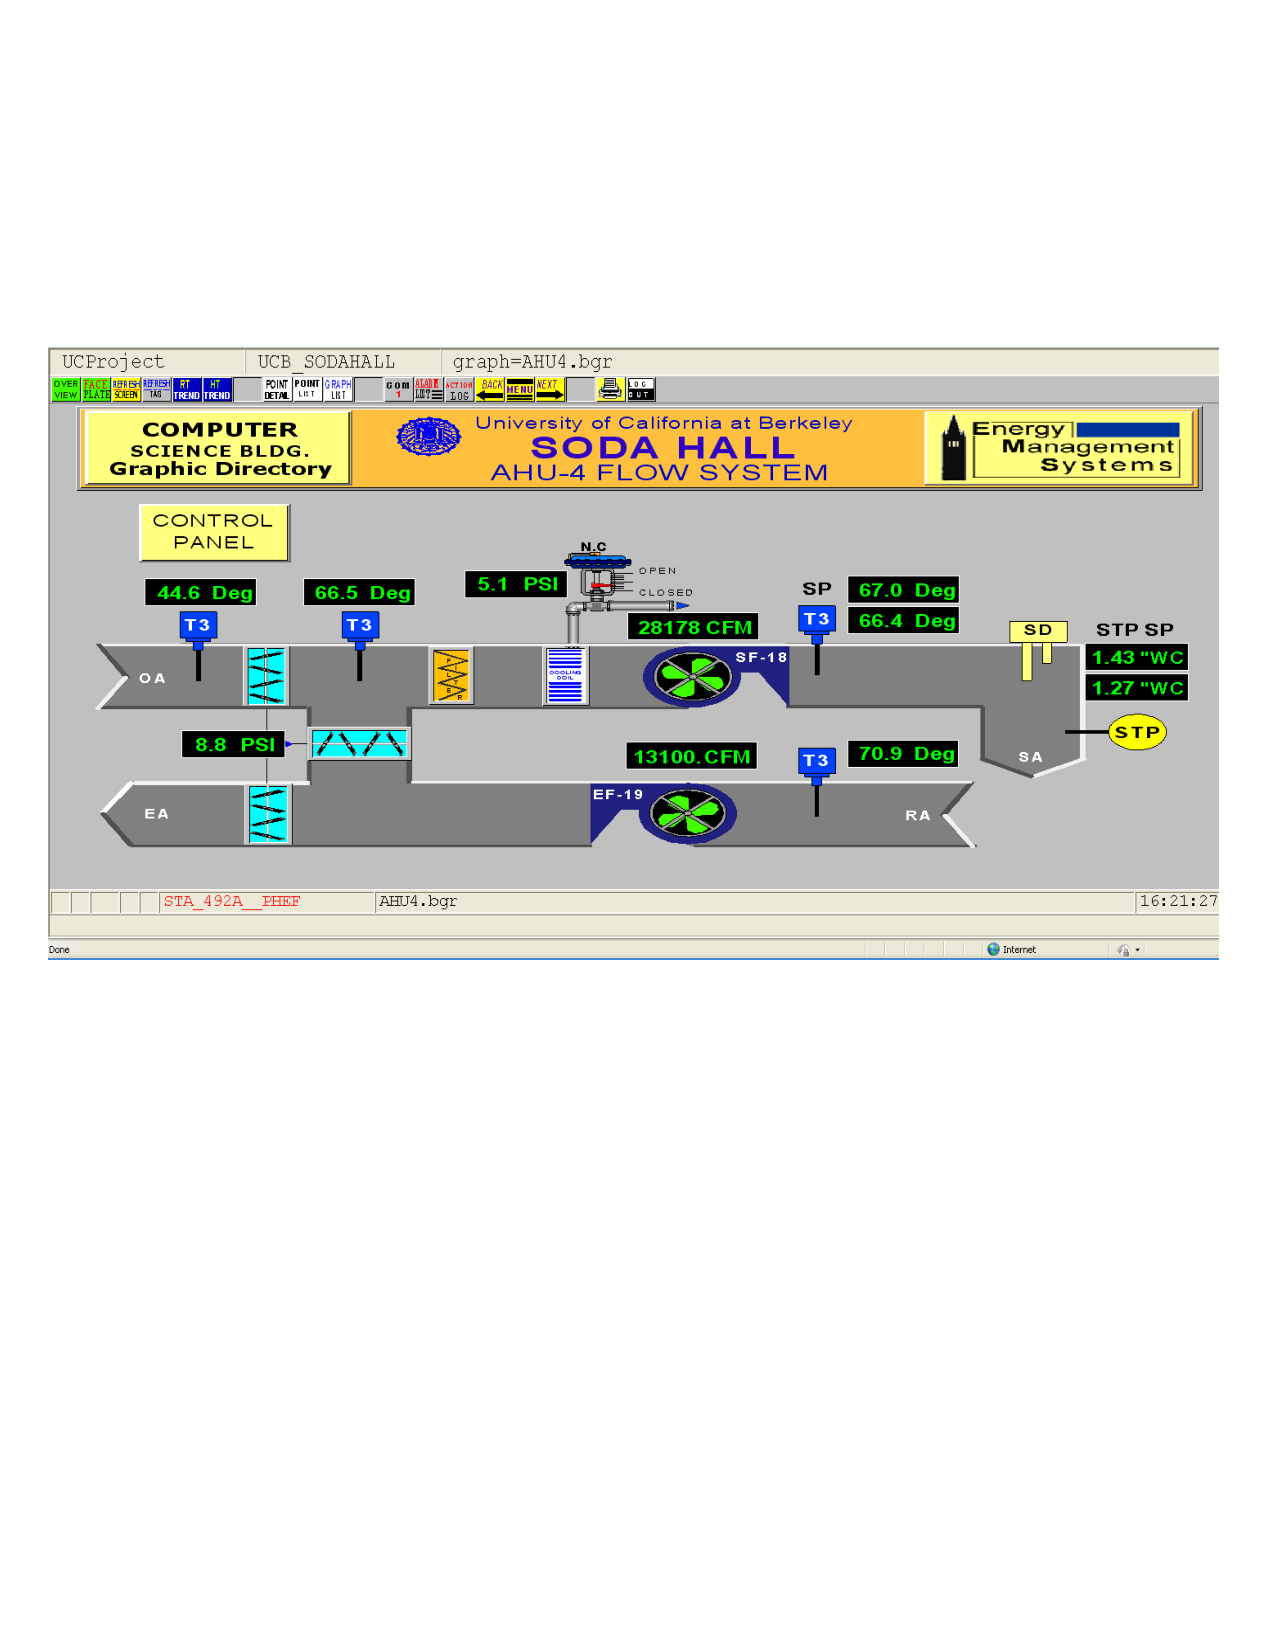
\includegraphics[width=0.75\columnwidth]{figs/soda_bms_screenshot}
\caption{Screen shot for the Soda Hall Building Management System Interface.}
\label{fig:soda_bms_screenshot}
\end{figure}

% In this section we dissect the current architecture in the context of current and future applications
% for buildings.  The first two describe how the current architecture is used to provide the intended service
% that these application provide.  The latter two are emerging applications that we would like to available
% throughout the entire building stock.  We will see, however, that these are very difficult to build at scale
% and we pose the question ``what is missing in the current architecture to enable the system properties that help
% support these and other emerging applications?''.  Through close inspection it will hopefully become clear that
% the current architecture is fundamentally flawed; built largely to support a small set of vendor-specific
% applications and not much else.

% In this section we dissect the BMS architecture and closely examine how well it can support broad application development
% in buildings, rather than the single supervisory control function it supports today.  
We examine today's BMS architecture in the context of 4 potential services with distinct operational requirements. % that need to be supported.  
The first two services are features in today's BMS's.  
We describe how emerging requirements are driving the evolution of these
services and how BMS's are struggling to meet the new requirements due to limitations in their architectural design.
The next two are emerging services that BMS's cannot support today.  We describe which architectural components must be included
or how current components must be modified in order to support these.  We also make the broader argument that 
building systems should be built to support a much wider range of applications that we cannot currently anticipate.
We will show why this requires a fundamental re-design and propose an architectural composition for such a system.
In the rest of the thesis, we will examine an instance of our architecture and describe the challenges in realizing
the use and effectiveness of our system in real building deployments.

% while the latter are potential applications we imagine will be supported in future
% smart buildings.  Through this exercise, we build our argument for a systematic re-design of such systems and propose
% a set of necessary architectural components necessary to enable and support emerging applications.

\subsection{Monitoring and Supervisory Control}
The primary objective in the design of building information systems is for centralized monitoring and supervisory
control.  Control algorithms are left ``to the expert'' and embedded in the outstation control board.  The intended
user of the system is a building manager -- a user whose expertise is much broader than the designer of the control
algorithm that runs on a particular system component.
The manager is expected to monitor the health of building systems and quickly diagnose problems when they occur.  The tool
is mainly in place to save the building manager time; and it is very effective at doing so.  The extent to which 
the building manager is making control decisions is altering control algorithm parameter setting through
the building management interface itself.  Even these decisions typically go through the vendor, through consultation.

Figure~\ref{fig:soda_bms_screenshot} shows a screenshot of the BMS in Soda Hall at UC Berkeley.  This specific image
captures a schematic for one of the air handling units.  It shows the various sensors embedded in different locations
on the component -- temperature sensors on either side of the supply/exhaust fans, temperature sensors at the supply/return 
air ducts and the inlet vent, measuring the outside air temperature.  Accompanying real-time readings are juxtaposed
by the sensor image.  The user can double-click on the sensor or reading to get more information about that particular 
measurement point.  For example, if you double-click on a temperature sensor, it will give you the exact name of the 
point and accompanying information about related points, such as the set-point, which effectively drives the behavior of 
the underlying system.  If an occupant makes a complaint about not getting any air from the vents, for example, the 
building manager can find the screen for the vents that serve the room the occupant is in and observe the current
pressure readings or look for value-based alerts on any of the readings, typically displayed on the same screen.
If there is a malfunctioning component or something stuck in the vent, the readings should ``look off'' to the building 
manager.

If the problem recurs often, the astute building manager may be able to characterize the fault through a series of alarms.
They can be proactive about finding and fixing the problem(s) before they occur.  Alarms can be set through interaction
with the graphical interface, in much the same way that a look up on the measurement point occurs -- by double-clicking on 
the point in question and following instructions for setting an alarm.  In some cases, the problem may be driven 
by a faulty setting and adjustments can be made to the control parameters through the associated control points.

The scope of control is limited to local control loops.  Recall our discussion of control loops in Section~\ref{sec:control_loops}.
The building manager can, typically with the help of the vendor, decide on the best control strategy setting.  If the control
strategy cannot be met, due to flaws in the control algorithm itself, the vendor may step in and re-image the controller
at the outstation and expose the necessary parameters through the graphical interface.  These kinds of changes are rare
but do happen occasionally and are generally expensive, since the cost is not usually included with the purchase
of the system.  The decision is made after close inspection and analysis, which a BMS enables through the data export feature.  
For example, the sense/control points in question may be placed in ``trend'' mode.  This means that readings
from those streams are stored in the local memory buffer at the outstation for some period of time.  If a report is specifically
set up at the central system, a report period is associated with the point of interest. This allows the saved data to be drained
from the local buffer at the outstation.  The data are written in a file for observation and graphing by the 
building manager.  %Time-dependent inspection of the behavior of any of the control-loop related points can be examined.

Although this feature is not necessary in order to change control parameters, it is useful for observing how parameter changes
affect the behavior of the system.  The building manager can, in principle, experiment with different setting and allow
empirical observations to guide her future decisions.


% Buildings waste as much as 30-80\% of their energy~\cite{waste_science, next10_waste}, have little agility
% to adjust to outside factor, and each one is unique from the mechanical system to the BMS.  This motivates
% the research presented in this thesis.  

\subsection{Energy Auditing and Building Modeling}
\label{sec:elensvision}
Recently there has been renewed interest in the energy consumption of buildings.  In particular, several studies~\cite{BuildingEnergyData,
MITBuildingScience} show that buildings consume a large fraction of the energy produced in the United States and that as much
as 80\% of it is wasted\cite{waste_science, next10_waste}.  As such, there has been an emergence of several companies and 
services for assessing the health of
commercial buildings with respect to their energy consumption.  Organizations such as LEED~\cite{Leed} provide certification of 
buildings, specifically rating the energy efficiency of the building.

Building modeling software, such as EnergyPlus~\cite{eplus}, are used extensively by building scientists. 
EnergyPlus and simulators like it are part of an ecosystem of software that models various aspect of the operation
of the building.  They allow the designer to construct detailed models of the building, from construction materials to 
operational usage and occupancy.  Some parameters include
construction material, longitude and latitude, zone-based usage (office building, bathroom, storage room), window size, etc.  
There are literally thousands of parameters that can be set.  All LEED certification relies on the construction of an 
accurate model that demonstrates energy efficient performance.
% Typical certification requires the submission of the detailed
% model and the results of various energy-related metrics, aggregated over seasonal time intervals to attain LEED certification.

Model construction can take several months.  In order to construct an accurate model, model output is compared with
empirical data.  Most BMS systems provide a way to export the  trended data.  
The file export feature and the ability to ``trend'' points, serve as an interface applications.
Another option is to obtain the data directly from the system through the network.  Third-party vendors provide systems that 
will join the building network of devices and eavesdrop on the network for sensor data reports.  % and traffic being reported to the central server.
In many instances, this is the only way to obtain truly real-time readings from the sensors on the network.
BMS vendors do not like this, since they such devices may generate traffic that overwhelms the network.  % because of congestion.
% Although not fundamental, it is a common concern in building sensor networks.  
Many buildings use RS-485 rather than Ethernet and there is
a general, albeit unfounded, concern that the network will become overwhelmed if all the points are trended and report 
simultaneously.

Modeling and real-time analysis have been separated because of these constraints.  The constraints are largely not
fundamental, but the current architecture is simply not designed to provide real-time readings for \emph{all the points, simultaneously}.
Also, it is clear, even from the fairly simple workloads generated by these analysis applications, that a history of readings
is needed.  BMS's, as currently designed, require the end-user to manage the history of the data point individually.
When BMS's were first designed, there were certainly concerns about bandwidth and storage limits.  However, today those concerns
are a non-issue.  A few hundred bytes produced on the order of minutes, even from several thousand sensors is simply not
that much data.  For example, 10k sensor produces readings every 15 minutes at 200 bytes per report is only 
17 Kbps.  Even if the streams are synchronized, the total amount of data is 2 MB.  Ethernet links and switches can handle Gbps 
transfers.


\subsection{Holistic Building Optimization}

\begin{figure}[t!] %htbp
\centering
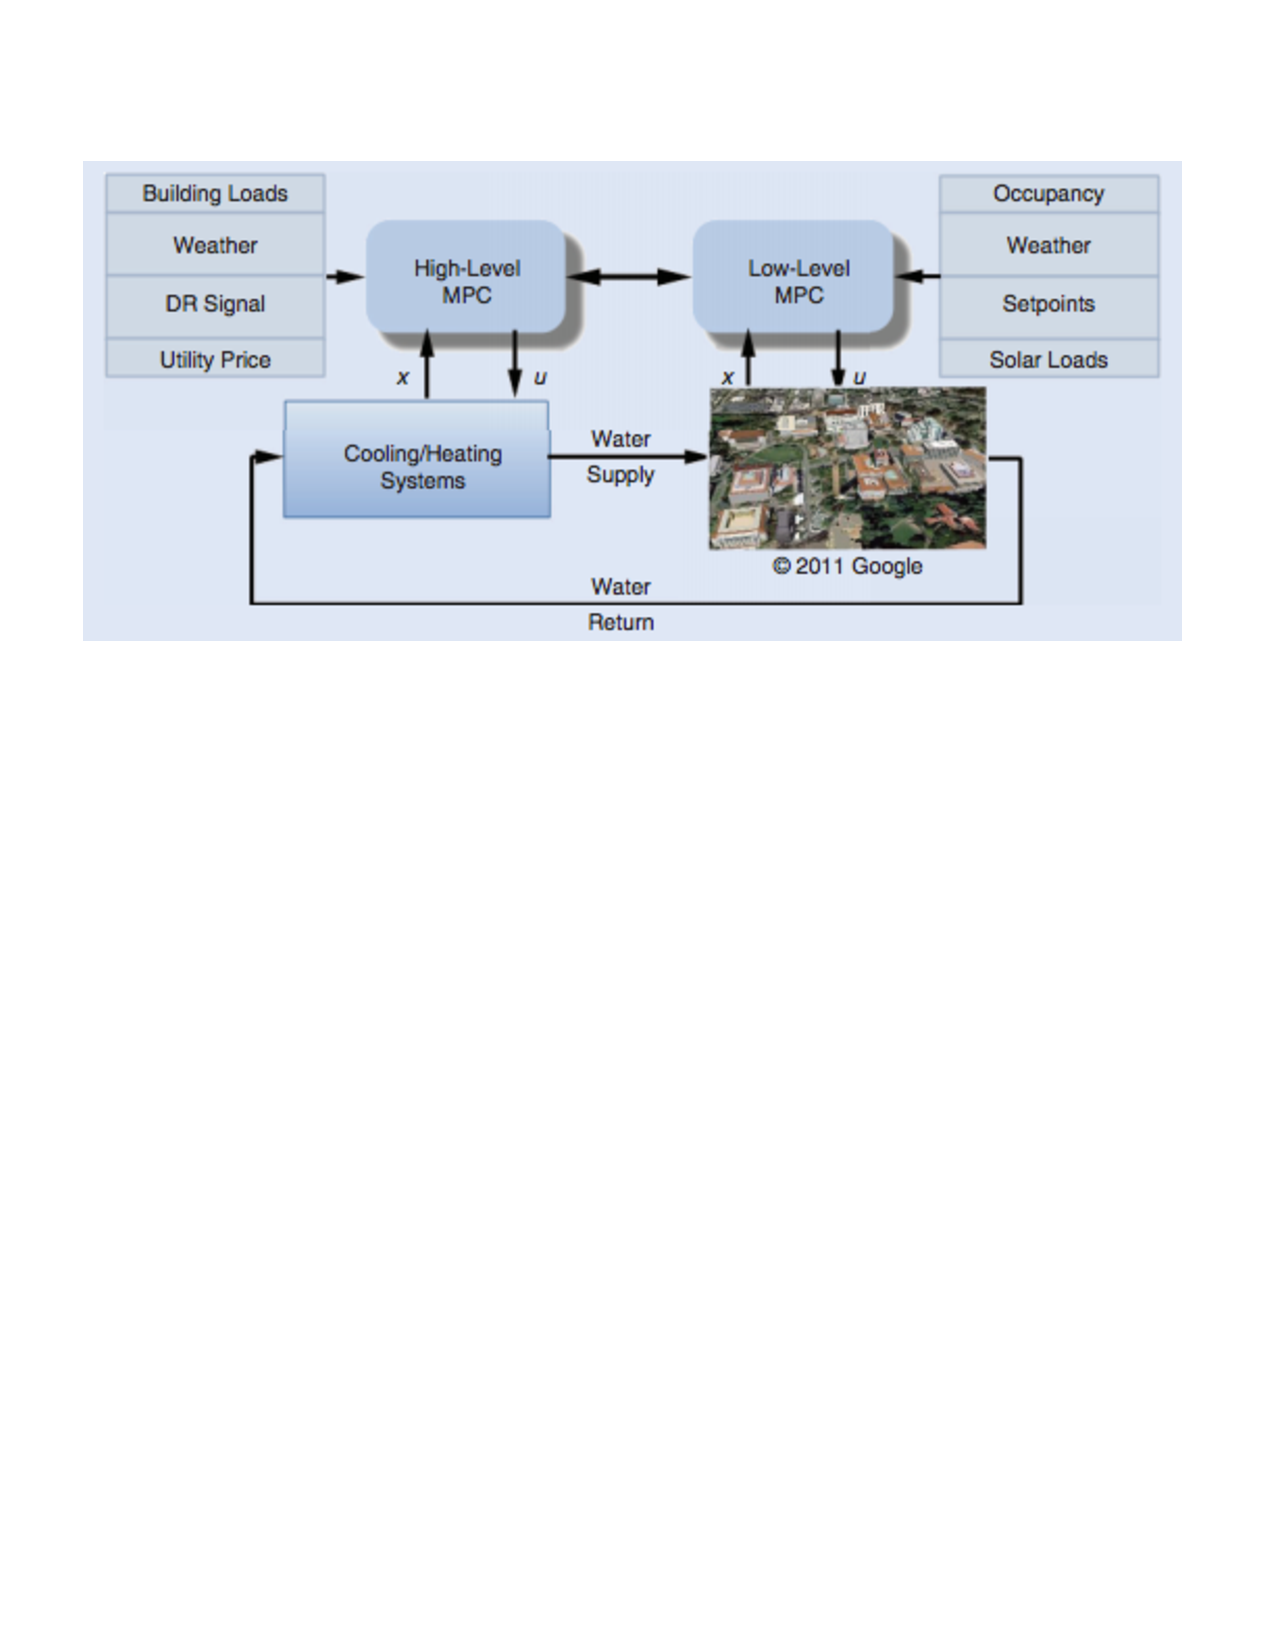
\includegraphics[width=0.75\columnwidth]{figs/mpc1}
\caption{Emerging Application: Hierachical MPC for a stock of buildings.}
\label{fig:mpc1}
\end{figure}

An emerging class of applications, is in holistic control of the building using a new technique called model-predictive control~\cite{MPC_yudong}.
Rather than rely on specific changes to control logic at the local-loop level, MPC techniques observe and learn a model
of the behavior of a components, multiple components, or the whole building, based on the historical data.  Once the model is learned, 
constraints can be specified to drive the behavior of the system to an optimal region in the trade off space; solving it as 
a constraint optimization problem.  Figure~\ref{fig:mpc1}, reproduced from~\cite{MPC_yudong}, shows an example of hierarchical MPC control.  
It decomposes a large optimization process -- High-level MPC --  into individual control decision to be made at the control-loop level --
low-level MPC.

In order to enable the low-level MPC, the process must know the mapping between the points and their location.
The user must connect the right data streams and control points to the algorithm's inputs by either manually going through the schematics or
locating the schematic representation in the BMS graphical interface.  There is no query interface to a BMS.  This task requires sitting 
with the building manager or vendor in order to set up the trending, reporting, and enabling the necessary control permisions.
Needless to say, it is very time consuming and \emph{does not scale}.

% Although the method is very useful and has yielded excellent results, it is difficult to replicate.   
% The code and setup must be 
% customized for each building or stock of buildings it is set up on.  
This lack of generalizability and scalability hinders widespread deployment of innovative solutions.  In most cases the 
mapping of sensor/actuator to their placement in space/system are 
captured through in a combination of the schematics, the graphical interface, and the point name. Moreover, buildings are 
are one-off constructions and their associated digital information has followed the same pattern.  Although MPC can yield significant savings, setup complexity and building uniqueness, makes it nearly impossible to replicate quickly.  It is fundamentally difficult to generalize. 


\subsection{Personal Energy Viewer}
\label{sec:mobile}

\begin{figure}[h!] %htbp
\centering
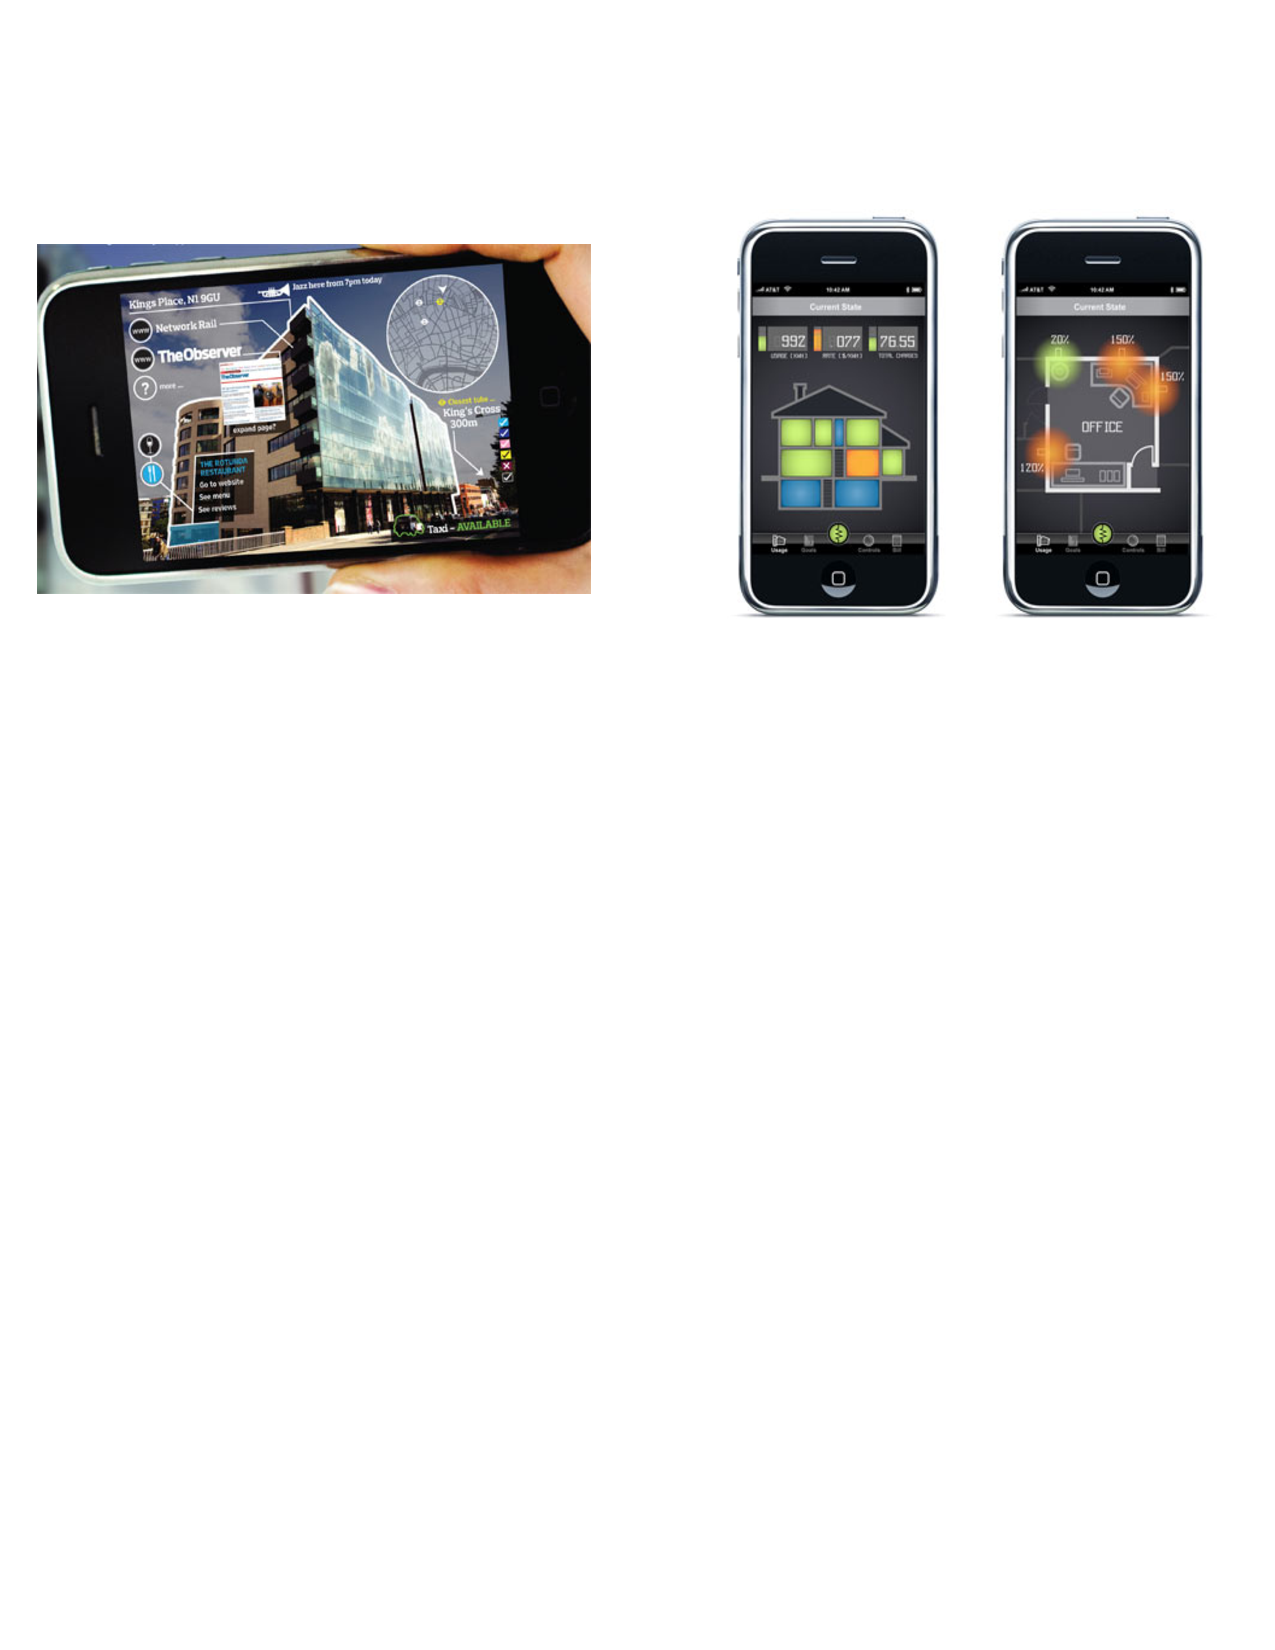
\includegraphics[width=0.75\columnwidth]{figs/mobileEnergy1}
\caption{Emerging Application: Mobile phone interfacing with the physical infrastructure.}
\label{fig:mobileEnergy1}
\end{figure}

Imagine having the ability to walk through a building and see live, detailed energy data as
you point your phone at various things and locations.  As you enter the building, you scan its tag and see
the live breakdown of energy consumption traces, including HVAC, lighting, and plug-loads.  You continue
your walk through the building as you head to your office.  When you arrive to your floor
you scan the tag for the floor and observe similar figures, only this time they are in relation to that floor
alone.  Since there are several meeting rooms on that floor, you are curious how much is consumed by 
occupants versus visitors.  You choose to view the total load curve co-plotted with the occupant
load curve, specifically for that floor.  You see that approximately half the total energy is consumed
by visitors during the day.  

Curious about what portion of total are attributed to you, you select the 
personalized attribution option and you see \emph{your} personal load curve plotted
with the total load curve -- as well as accompanying statistics, such as the percent of total over time.
As you quickly examine the data on your phone, you see that you consumed energy during hours that you were not
there.  You choose to see a more detailed breakdown.  You enter your office, scan various items that you own, and see that
your computer did not shut down properly and your light switch was set to manual.  You immediately 
correct these.

Being able to interact with your environment and get a complete energy break-down can provide a useful tool
for tracing and correcting rampant energy consumption.  In buildings, having the occupants actively participate
allows for localized, personal solutions to efficiency management and is crucial to scaling to large buildings.
However, providing this detailed level of attribution is challenging.  There's lots of data coming from various systems 
in the building, and integrating them in real time is difficult.  Furthermore, attribution is non-trivial.  
We must be able to answer to following: How much of the total consumed on this floor went to charging laptops?  How
many of those charging laptops belong to registered occupants of this floor?
For centralized systems, multiple locations are served simultaneously.  It is non-trivial to determine the exact
break-down for each location.  At the plug-load level, some plug loads move from place to place throughout the building
over the course of the day.  Tracking where they are at any given time is difficult.

Answering these queries is relatively easy once the information is available, however, collecting the information
is non-trivial, especially over time.  Historically, it has been difficult to collect plug-load information.
Various studies have used wireless power meters to accomplish just this~\cite{stephscale, lanz, aceee}.
All previous work collected the data and performed post-processing to analyze it.  We want to take the next
natural set of steps: perform processing in real-time and present the occupants with live information.

Currently, in order to enable this application, a detailed digital model of the building is necessary, data streams from the building must
be easy to query, and it should work across buildings.  Also, there needs to be a way to localize the user. 
Localization technology and information must be made available to the mobile application to provide in-situ services.
It's clear that the current information infrastructure cannot provide these.  The interface to the network does not have
a strict naming mechanism, there is not explicit representation of each building that the application could interpret, 
the sensor/actuator deployment is not dense enough and adding new sensor is cumbersome.  Furthermore, the data itself can be quite dirty.

Cheap sensors are unreliable.  They produce erroneous data and randomly stop and start at times.  Missing/erroneous data is common.
Moreover, within building information systems provided by a single vendor, there is no time synchronization across sensors, so
aggregation, filtering, and re-sampling are common operations that must be performed on the data in order to summarize and display it.
The mobile energy viewer application not only require these but requires that they be performed in real time.




